%instiki:category: FisicaSubatomica
\chapter{Ruptura espont\'anea de simetr\'\i a}
\label{rupt-espont-de} %noinstiki
%instiki:
%instiki:***
%instiki:
%instiki:[[NotasFS|Tabla de Contenidos]]
%instiki:
%instiki:***
%instiki:
%instiki:* [Masa para el campo escalar](#masa-para-el)
%instiki:
%instiki:* [Bos\'on de Goldstone](#boson-de-goldstone)
%instiki:
%instiki:* [Masa para el bos\'on gauge](#masa-para-el-1)
%instiki:
%instiki:* [Mecanismo de Higgs en un caso no Abeliano](#mecanismo-de-higgs)
%instiki:
%instiki:***
%instiki:


\section{El resurgimiento del éter.}

Tomado de~\cite{restrepo2013resurgimiento}.

%slides in juevesdelaciencia.pdf pag. 35

  La superconductividad electromagnética puede usarse como una analogía bastante precisa para aclarar muchos aspectos del mecanismo de Higgs en las interacciones débiles y  entender la relevancia del descubrimiento de la nueva partícula encontrada recientemente en el Gran Acelerador de Hadrónes (LHC de sus siglas en inglés).  Dentro de un \emph{superconductor electromagnético} la luz se propaga a través de un éter del que se conoce su composición y propiedades. El universo en su totalidad puede entenderse como un enorme \emph{superconductor débil} del que estamos comenzando a dilucidar sus propiedades.


Existe una analogía muy precisa entre el mecanismo de Higgs y la superconductividad a bajas temperaturas. No en vano el propio mecanismo de Higgs surgió de explotar esa analogía (ver el artículo de D. Portillo en estas memorias). El descubrimiento reciente de una partícula con las propiedades esperadas para el Higgs, apunta al resurgimiento del concepto de  un éter que permea todo el universo asociado con las interacciones débiles, una de las cuatro interacciones fundamentales de la naturaleza~\cite{pi} responsable del decaimiento de los núcleos radiactivos. En este trabajo se explicará como incluso el escurridizo éter lumínico ha encontrado cabida en algunos rincones muy especiales de la naturaleza, donde se ha logrado obtener la superconductividad electromagnética.   

El éter lumínico había surgido de la necesidad mecanisista de dotar al universo de un medio a través del cual se pudiesen propagar las ondas electromagnéticas. Esta visión del mundo quedó poco a poco reemplazada por la visión más simple de la relatividad espacial basada en el postulado de que las leyes de la física deben ser las mismas para todos los observadores que se muevan a velocidad constante. Aunque en la formulación inicial de la relatividad especial no quedó para nada explícito, nuestro entendimiento actual de la naturaleza del espacio y el tiempo esta estrechamente ligado con la existencia de una velocidad límite que no puede ser superada por ningún cuerpo material ni por ningún tipo de información~\cite{0708.0929}. Una partícula sin masa viaja a dicha velocidad límite, independiente de la velocidad que tenga su observador. Así mismo, si se puede determinar con suficiente precisión que la velocidad de un cuerpo es la misma independiente de la velocidad del observador, entonces necesariamente ese cuerpo debe viajar a la velocidad límite. La identificación de la velocidad límite con la velocidad de la luz es un resultado experimental sujeto a constante verificación. Cualquier desviación experimental que se encuentre al respecto podría ser evidencia de que las partículas que componen la luz tienen alguna masa.

Como la masa ha resultado ser un concepto emergente en la física moderna, la posibilidad de que las partículas que componen la luz tengan o no masa, depende de la interacción de dichas partículas con el medio en el que se propagan. Contrario a lo que se suele establecer usualmente, el resultado negativo del experimento de Michelson y Morley \cite{EMM} no implica que no existe un éter; implica que de existir un éter, la luz no interacciona con él. La presencia de otros tipos de luz, asociadas con interacciones diferentes a la electromagnética, podría hacer manifiesta la presencia de ese éter.  Aún más, la existencia misma de un éter lumínico podría manifestarse bajo otras condiciones diferentes a la usuales, como por ejemplo, a temperaturas cercanas al cero absoluto y dentro de cierto tipo de materiales.

De hecho, el resurgimiento del éter sucedió casi de inmediato con el descubrimiento de la \emph{superconductividad electromagnética} en 1911. La superconductividad electromagnética es la desaparición de la resistencia eléctrica que ocurre en algunos materiales cuando se disminuye su temperatura por debajo de algún valor crítico. La conducción de corriente eléctrica a través de un alambre superconductor es mucho más eficiente y permite generar campos magnéticos mucho más intensos que los que se obtendrían con materiales conductores convencionales a partir de  la misma cantidad de energía. Además, un material superconductor tiene la propiedad de repeler los campos magnéticos externos a él. El piso de un vagón repleto de pasajeros hecho de un material superconductor, puede levitar sobre rieles imantados, como ocurre con los trenes de levitación magnética del tipo JR-Maglev en Japón~\cite{maglev}. 

El entender la superconductividad no fue inmediato porque es un proceso cuántico en el que convergen mucho conceptos teóricos desarrollados posteriormente. Un sistema cuántico como un núcleo, un átomo, una molécula, etc; tiene niveles de energía discretos que pueden ser ocupados secuencialmente dependiendo de si las partículas que interaccionan con el sistema son \emph{bosones} o \emph{fermiones}.  Los fermiones tienen una cantidad de movimiento angular intrínseco, llamado espín, en unidades semienteras de la constante de Planck reducida, denotada por $\hbar$ (la cual caracteriza los fenómenos cuánticos). Los bosones, de otro lado, tienen espín en unidades enteras de $\hbar$. La contraparte clásica del espín corresponde a la cantidad de movimiento angular de una esfera en rotación sobre un eje, determinada por el producto entre su momento de inercia\footnote{El momento de inercia de una esfera uniforme de radio $R$ y masa $M$, alrededor de un eje que pasa por su centro es $2MR^2/5$. El ``espín'' de la tierra es del orden de $10^{67}\hbar$.} y su velocidad angular. La forma en que los fermiones pueden ocupar los niveles de energía esta restringido por el principio de exclusión de Pauli, que establece que un mismo nivel de energía no puede ser ocupado por dos o más fermiones con los mismos números cuánticos. El fermión más simple es el electrón que tiene como números cuánticos la carga eléctrica (de menos uno en unidades de la propia carga del electrón) y el espín que puede ser $\hbar/2$ o $-\hbar/2$. El nivel de energía fundamental de un átomo de Helio puede ser ocupado a lo sumo por dos electrones de espines opuestos. Siguiendo toda la secuencia de átomos,  el Principio de exclusión de Pauli permite explicar la estructura de la tabla periódica de los elementos químicos. 

Se ha logrado establecer que un metal esta conformado por una estructura cristalina, la cual también exhibe niveles de energía cuánticos cerca a su superficie. Los electrones de valencia  de cada átomo, es decir los electrones del último nivel de energía atómico, pueden ocupar los niveles de energía del cristal moviéndose a través de toda su superficie. El movimiento colectivo de los electrones de valencia se comporta como un fluido de cierta profundidad que se llama mar de Fermi. Como en el mar, las profundidades son tranquilas y toda la activad sucede en la superficie del mar de Fermi. Un rayo de luz puede viajar a través del mar de Fermi sin prácticamente interaccionar con él, manteniendo una velocidad muy cercana a la velocidad límite de la relatividad especial.

Es bien conocido que dos cargas eléctricas de signos opuestos se atraen, mientras que cargas del mismo signo se repelen. Sin embargo, cuando un metal se enfría por debajo de una temperatura crítica, puede ocurrir el fenómeno sorprendente de que dos electrones se puedan atraer entre sí. A bajas temperaturas, las oscilaciones de la estructura cristalina se estabilizan y los átomos del metal empiezan a ocupar posiciones bastante fijas en el espacio. Cada átomo del metal es visto por un electrón de valencia como un ion de carga positiva y por consiguiente lo atrae creando una acumulación de carga positiva alrededor de él como se muestra en la Figura~\ref{fig:1}(a) adaptada de \cite{beamline}.  En la figura~\ref{fig:1}(b) se muestra  el efecto de polarización de la red cristalina que corresponde a una acumulación de carga positiva alrededor del punto donde se encuentra el electrón de valencia. Cuando otro electrón de valencia se acerca a la zona polarizada por el primer electrón,  siente una atracción neta hacía ese sitio. El efecto total es que dos electrones de espines opuestos se pueden atraer lo suficiente como para formar un estado ligado llamado par de Cooper. Al estar formado por pares de electrones de espines opuestos, el espín del par de Cooper es cero, y corresponde a un  bosón que ya no está restringido por el principio de exclusión de Pauli. El par de Cooper entonces se puede sumergir en las profundidades mar de Fermi hasta ocupar el nivel de energía fundamental. Al final, después de que todos los electrones de valencia se han apareado, todos ellos se \emph{condensan} en el nivel de energía fundamental.

\begin{figure}
  \centering
  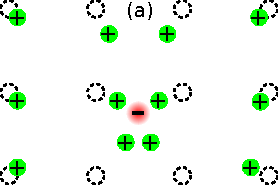
\includegraphics{metalcristal1}\hspace{4cm}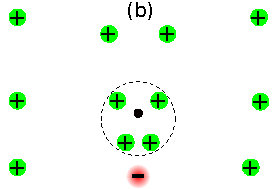
\includegraphics{metalcristal2}
  \caption{En la figura (a), los círculos con líneas a trazos representan las posiciones originales de los iones positivos en el cristal. Debido a la presencia del electrón de valencia, el cristal se polariza y se genera un exceso de carga positiva alrededor del electrón que resulta entonces apantallado. En la figura (b) se muestra como el exceso de carga positiva puede causar un efecto de atracción sobre otro electrón de valencia lo que permite la formación de un par de Cooper.}
  \label{fig:1}
\end{figure}

Este tipo de condensados de bosones, que ocurren por debajo de una cierta temperatura crítica, tiene todas las características de un éter lumínico: cuando la luz se propaga a través del condensado adquiere una masa emergente que hace que su velocidad sea menor que la velocidad límite de la relatividad especial. Esta nueva velocidad ya si depende de la velocidad del observador que la mida. Si se pudiese repetir el experimento de Michelson y Morley dentro de un superconductor: ¡daría un resultado positivo!

Pero, ¿cómo es posible que un fotón adquiera inercia?. Al tiempo en el que Clerk Maxwell estableció las ecuaciones del electromagnetismo, ya se conocía la Ley de Faraday que establece que los campos eléctricos en movimiento (las corrientes eléctricas) producen campos magnéticos. Usando principios de simetría, Maxwell completo las leyes electromagnéticas prediciendo que los campos magnéticos en movimiento producen también campos eléctricos. Como los campos eléctricos en movimiento producen campos magnéticos en movimiento, que a su vez producen de nuevo campos eléctricos en movimiento, entonces se genera un movimiento ondulatorio y las ecuaciones de Maxwell automáticamente predicen la existencia de ondas electromagnéticas. Una consecuencia inmediata es que la luz visible es simplemente un tipo especial de onda electromagnética en un rango de frecuencias determinado. Una onda electromagnética se puede representar entonces con un vector oscilante que representa el campo magnético, asociado con otro vector oscilante y perpendicular de campo eléctrico. La luz se propaga a la velocidad límite de la relatividad especial en una dirección perpendicular al plano definido por los dos vectores como se ilustra en la figura~\ref{fig:2}(a). Cuando la onda electromagnética se propaga dentro de un condensado sobre la superficie de un superconductor, una componente del par de Cooper se puede acoplar a los vectores magnético y eléctrico en la dirección de propagación de la onda, causando un efecto de frenado. En el lenguaje de la ruptura espontánea de simetría, que explica la formación del condensado por debajo de una temperatura crítica, se dice que fotón se come una componente del par de Cooper para así adquirir masa, como se muestra en la figura~\ref{fig:2}(b). Una vez la luz adquiere masa, las interacciones electromagnéticas se convierten en interacciones de rango finito. Es decir, que a partir de cierta separación entre las cargas eléctricas dentro de un superconductor, desaparecen las fuerzas eléctricas entre ellas. Aunque cuantitativamente estos efectos son pequeños pues la masa del fotón dentro de un superconductor es del orden de una billonésima de electron-voltio~\cite{beamline} (similar a las masas de neutrinos), cualitativamente el comportamiento cambia drásticamente: se pasa de una interacción de rango infinito mediada por fotones de masa cero, a una interacción de \emph{alcance restringido} mediada por fotones masivos. 

\begin{figure}
  \centering
  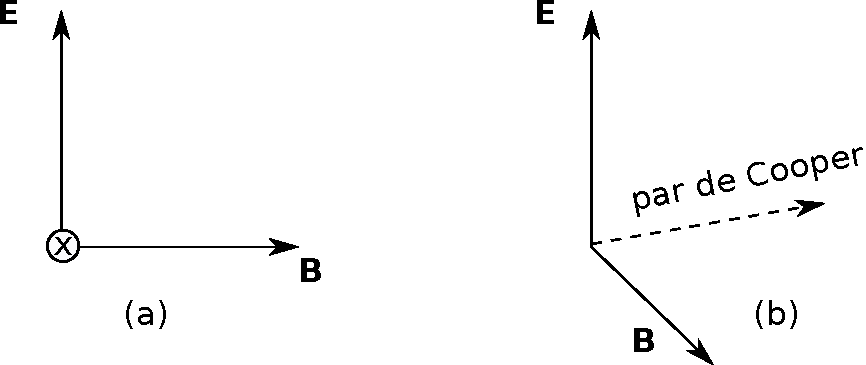
\includegraphics[scale=0.7]{ondaEM}
  \caption{En la figura (a), se representa los campos eléctricos y magnéticos de una onda electromagnética propagándose a la velocidad de la luz en una dirección entrando a la hoja. En  la figura (b) se muestra una onda electromagnética propagándose dentro de un condensado de pares de Cooper, en la dirección de la componente ilustrada del par de Cooper.}
  \label{fig:2}
\end{figure}


Cuando se calienta un superconductor metálico por encima de su temperatura crítica correspondiente a unos pocos grados kelvin sobre el cero absoluto, todo vuelve a la normalidad. El estado no superconductor es más simétrico porque los electrones del mar de Fermi están orientados en todas direcciones. El estado superconductor representa un estado menos simétrico pues todos los pares de Cooper están orientados formando un estado coherente en una dirección específica del espacio. Al formarse el condensado se da un fenómeno de \emph{ruptura espontánea de la simetría}: las simetrías iniciales que describen las interacciones del sistema se mantienen, pero el estado fundamental rompe la simetría.  

El electromagnetismo es la interacción mejor conocida de las cuatro interacciones fundamentales~\cite{pi}. Las interacciones fundamentales  entre partículas están mediadas por cierto conjunto de bosones.  Es así como la interacción electromagnética entre partículas cargadas, esta mediada por los fotones. Las interacción fuerte, que mantiene unidos de forma estable los componentes de los núcleos atómicos, está mediada por los gluones, los cuales tampoco requieren un medio para propagarse. La fuerza fuerte es en muchos otros aspectos similar a la fuerza electromagnética. 

Sin embargo, las interacciones débiles han resultados ser fuerzas de corto alcance, mediadas por nuevos fotones llamados $W$ y $Z$ que son bastante masivos: del orden de cien veces la masa del protón. La pregunta de si esas masas son reales o emergentes, se reduce a descubrir la existencia del éter a través del cual se propagan esas nuevas ondas débiles. Aunque no podemos acceder directamente a las componentes del condensado que se comen el $W$ y el $Z$ para adquirir masa, existe al menos otra componente del condensado que se debe materializar como partícula independiente y nueva: la partícula de Higgs. 

De confirmarse que la partícula recientemente descubierta en el Gran Acelerador de Hadrónes (LHC de sus siglas en inglés) corresponde al Higgs, significaría nada más y nada menos que el universo se encuentra en un estado de superconductividad débil (\emph{superconductividad electródebil para ser más exactos.}) El universo en su totalidad es un superconductor en el sentido de que las partículas que sólo tienen cargas débiles como los neutrinos, viajan por la materia sin mayor resistencia. De hecho nuestro cuerpo, e incluso el planeta entero, están siendo atravesados constantemente por neutrinos\footnote{Y por las supuestas partículas de materia oscura débilmente interactuantes, aunque estas aún no ha dejado trazas ni siquiera en los diversos experimentos de detección directa instalados en varios laboratorios subterráneos de la Tierra.}. Para hallar las excitaciones del éter débil, correspondientes a la partícula de Higgs, debemos calentar al menos una porción del universo por encima de la temperatura crítica de la ruptura espontánea de simetría electrodébil estimada en un cuadrillón de grados kelvin ($10^{15}\ $K). Eso es precisamente lo que se está haciendo el LHC en los puntos de colisión de los detectores ATLAS y CMS~\cite{quarknet}, de donde al parecer están emergiendo las primeras partículas de Higgs. 

 



\section{Campo escalar real}
Escribamos el Lagrangiano para una part\'\i cula escalar real de masa $m$ como
\begin{equation}
\label{eq:83qft}
\mathcal{L}=\tfrac{1}{2}\partial^\mu\phi\partial_\mu\phi-V(\phi)
\end{equation}
con
\begin{equation}
  V(\phi)=\tfrac{1}{2}\mu^2\phi^2.
\end{equation}
Este Lagrangiano es simétrico bajo la transformación discreta $\phi\to-\phi$. 

Cuando $\mu^2\gt 0$, el campo tiene excitaciones alrededor del mínimo del potencial que cuestan energía y dicho término se interpreta como la masa de la partícula. Ver figura \ref{fig:x2}. En Teoría Cuántica de Campos al estado de mínima energía se le llama el vacío y las excitaciones alrededor del vació corresponden a las partículas.
%noinstiki
\begin{figure} %noinstiki
  \centering %noinstiki
  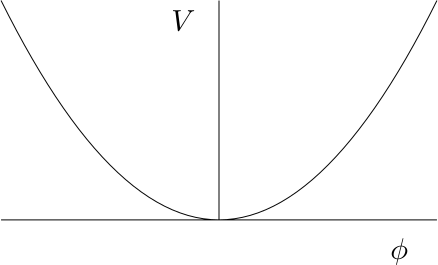
\includegraphics[scale=0.8]{vphi2}
  \caption{$V(\phi)=\frac{1}{2}\mu^2 \phi^2$ con $\mu^2\gt 0$} %noinstiki
  \label{fig:x2} %noinstiki
\end{figure} %noinstiki <div id="fig:x2">Figura: Un mínimo</div>
%noinstiki![cuerda](http://gfif.udea.edu.co/figfs/vphi2.png)
%noinstiki

Si $\mu^2\lt 0$, no existe un mínimo del potencial alrededor del cual el campo pueda oscilar. Además el alejamiento del campo del punto de simetría del potencial no cuesta energía. Por consiguiente en ese caso, el término de interacción
\begin{equation}
  V(\phi)=\tfrac{1}{2}\mu^2   \qquad 
  \mu^2\lt 0,
\end{equation}
no puede interpretarse como un término de masa en el Lagrangiano dado por la ec.~\eqref{eq:83qft}. 

Consideremos ahora el potencial
\begin{equation}
  V(\phi)=\tfrac{1}{2}\mu^2\phi^2+\tfrac{1}{4}\lambda\phi^4
  \qquad   \mu^2\lt 0,\ \lambda\gt 0
\end{equation}
que mantiene la simetría bajo la transformación discreta $\phi\to-\phi$. $\lambda\gt 0$ garantiza la aparición de los dos mínimos que se muestran el la figura \ref{fig:x2l}. Si la energía es suficientemente alta como se muestra en la figura~\ref{fig:x2l}, las excitaciones son simétricas con respecto al máximo del potencial y el término en $\mu^2$ no puede interpretarse como masa para la partícula escalar. 

%noinstiki
\begin{figure} %noinstiki
  \centering %noinstiki
  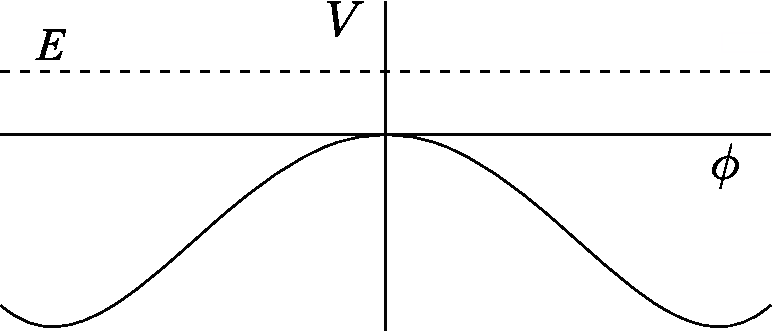
\includegraphics{vphi4}
  \caption{$V(\phi)=\frac{1}{2}\mu^2 \phi^2+\frac{1}{4}\lambda\phi^4$ con $\mu^2\lt 0$, y $\lambda\gt 0$. Simetría exácta} %noinstiki
  \label{fig:x2l} %noinstiki
\end{figure} %noinstiki <div id="fig:x2l">Figura: Mínimos degenerados</div>
%noinstiki![cuerda](http://gfif.udea.edu.co/figfs/vphi4.png)
%noinstiki
Sin embargo, si la energía es suficientemente baja como se muestra en la figura~\ref{fig:x2lm}, las excitaciones alrededor del mínimo dan lugar a la aparición de un término de masa para el campo escalar. Además, dichas excitaciones no respetan la simetrías $\phi\to-\phi$. En tal caso decimos que la simetría ha sido espontáneamente rota: aunque el Lagrangiano mantiene la simetría original, el vacío la rompe. 

%noinstiki
\begin{figure} %noinstiki
  \centering %noinstiki
  %noinstiki
  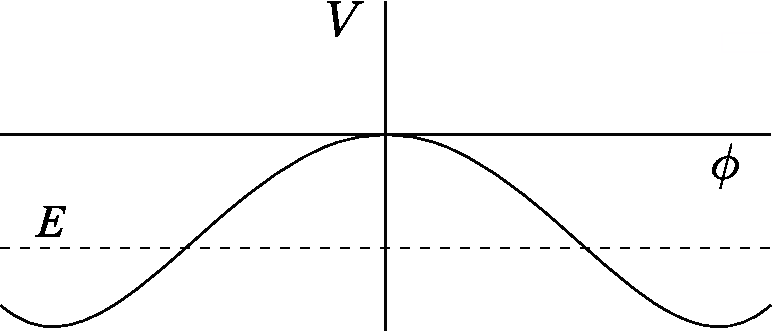
\includegraphics{vphi4m}
  \caption{$V(\phi)=\frac{1}{2}\mu^2 \phi^2+\frac{1}{4}\lambda\phi^4$ con $\mu^2\lt 0$, y $\lambda\gt 0$. Simetría espontáneamente rota.} %noinstiki
  \label{fig:x2lm} %noinstiki
\end{figure}  %noinstiki <div id="fig:x2lm">Figura: Simetría espontáneamente rota  </div>
%noinstiki![vphi4lm](http://gfif.udea.edu.co/figfs/vphi4lm.png)
%noinstiki

Para analizar cuantitativamente el espectro de partículas es necesario expandir el campo alrededor del mínimo y determinar las excitaciones. Establezcamos en primer lugar los mínimos del potencial. La $\partial V/\partial\phi=0$ da lugar a
\begin{align}
  \mu^2\phi+\lambda\phi^3&=0\\
  \phi(\mu^2+\lambda\phi^2)&=0,
\end{align}
con extremos $\phi_{\text{max}}=0$, y 
\begin{equation}
  \label{eq:90qft}
  \phi_{\text{min}}\equiv\langle\phi\rangle\equiv v=\pm\sqrt{\frac{-\mu^2}{\lambda}}.
\end{equation}
De hecho 
\begin{equation}
  \frac{\partial^2V}{\partial\phi^2}=\mu^2+3\lambda\phi^2.
\end{equation}
$\phi=0$ corresponde a un máximo, mientras que la segunda derivada para $\phi=\pm\sqrt{-\mu^2/\lambda}$ es $-2\mu^2\gt 0$ y corresponden a los mínimos. Expandiendo el campo alrededor del mínimo
\begin{equation}
  \phi(x)=H(x)+v
\end{equation}
\begin{align}
  V(\phi)=&\tfrac{1}{2}\mu^2 \phi^2+\tfrac{1}{4}\lambda\phi^4\nonumber\\
  =&\tfrac{1}{2}\mu^2 (H+v)^2+\tfrac{1}{4}\lambda(H+v)^4\nonumber\\
  =&\tfrac{1}{2}\mu^2 (H+v)^2+\tfrac{1}{4}\lambda(H+v)^4\nonumber\\
  =&\tfrac{1}{2}\mu^2 \left(H^2+2vH+v^2\right)+\tfrac{1}{4}\lambda\left(H^2+2vH+v^2\right)^2\nonumber\\
  =&\tfrac{1}{2}\mu^2 \left(H^2+2vH+v^2\right)+\tfrac{1}{4}\lambda\left[H^4+2H^2\left(2vH+v^2\right)+\left(2vH+v^2\right)^2\right]\nonumber\\
  =&\tfrac{1}{2}\mu^2 \left(H^2+2vH+v^2\right)+\tfrac{1}{4}\lambda\left[H^4+4vH^3+2H^2v^2+4v^2H^2+4v^3H+v^4\right]\nonumber\\
  =&\tfrac{1}{2}\mu^2 \left(H^2+2vH+v^2\right)+\tfrac{1}{4}\lambda\left[H^4+4vH^3+6H^2v^2+4v^3H+v^4\right]\nonumber\\
  =&\tfrac{1}{2}\mu^2H^2-\tfrac{3}{2}H^2\mu^2+\mu^2vH-\mu^2vH+\tfrac{1}{2}\mu^2v^2-\tfrac{1}{4}\mu^2v^2+\tfrac{1}{4}\lambda\left[H^4+4vH^3\right]\nonumber\\
\label{eq:84qft}
V(H)=&\tfrac{1}{2}\left(-2\mu^2\right)H^2+\lambda vH^3+\tfrac{1}{4}\lambda H^4+\tfrac{1}{4}\mu^2v^2,
\end{align}
y
\begin{equation}
  \label{eq:88qft}
  \mathcal{L}_H=\tfrac{1}{2}\partial^\mu H\partial_\mu H-\tfrac{1}{2}\left(-2\mu^2\right)H^2-\lambda vH^3-\tfrac{1}{4}\lambda H^4+\text{constant}.
\end{equation}
Entonces $H$ adquiere una masa $-2\mu^2$ y no es invariante bajo $H\to-H$. 

Otro método es usar las ecuaciones de mínimo $-\mu^2=\lambda v^2$, para eliminar un parámetro del potencial:
\begin{align}
  V(\phi)&=-\tfrac{1}{2}\lambda v^2\phi^2+\tfrac{1}{4}\lambda\phi^4\nonumber\\
  =&-\tfrac{1}{2}\lambda v^2 \left(H^2+2vH+v^2\right)+\tfrac{1}{4}\lambda\left[H^4+4vH^3+6H^2v^2+4v^3H+v^4\right]\nonumber\\
  =&\lambda v^2H^2+\lambda vH^3+\tfrac{1}{4}\lambda H^4+\text{constant}.
\end{align}
Podemos escribir el potencial en términos del  nuevo campo como
\begin{align}
\label{eq:higgspot}
  V(H)=\frac{1}{2}m_H^2H^2+\frac{1}{2}\frac{m_H^2}{v}H^3+\frac{1}{8}\frac{m_H^2}{v^2} H^4\,.
\end{align}
donde
\begin{equation}
\label{eq:higgsmass}
  m_H^2=2\left|\mu^2\right|=2\lambda v^2
\end{equation}

\subsection{Ausencia de taquiones}

Uno se podría preocupar por la presencia de un término de masa
imaginaria en el Lagrangiano, pero como estamos hablando de
transiciones de fase, estos porcesos deben suceder en presencia de
temperatura, por ejemplo la temperatura asociada al universo primitivo
durante las fases tempranas del Big Bang. En presencia de temperatura,
todas las partículas adquieren una masa térmica proporcional a la
temperatura como resultado de su interacción con el plasma. De este
modo, a altas temperaturas la masa de la partícula escalar esta
dominada por la temperatura y al ser positiva el potencial escalar
tiene un único mínimo simétrico. Cuando la temperatura baja lo
suficiente para que la masa al cuadrado negativa domine, el mínimo se
convierte en un máximo local altamente inestable y ocurre muy
rapidamente la transición de fase al nuevo mínimo no simétrico donde
la masa del escalar esta bien definida.

\subsection{Caso complejo}


Consideremos ahora un campo escalar complejo sin término de masa, pero con potencial:
\begin{equation}
  \label{eq:85qft}
  \mathcal{L}=\partial^\mu\phi^*\partial_\mu\phi-V(\phi)
\end{equation}
\begin{equation}
  V(\phi)=\mu^2\phi^*\phi+\lambda(\phi^*\phi)^2 
  \qquad 
  \mu^2\lt 0,\ \lambda\gt 0 
\end{equation}
La simetría del Lagrangiano corresponde a $U(1)$ global. Este potencial corresponde al ``sombrero mexicano'', como se ilustra en la Figura \ref{fig:mexicanhat}. Para una energía suficientemente baja de manera que el campo deba oscilar alrededor del mínimo aparecen dos tipos de excitaciones. Una sobre las paredes  que cuestan energía y corresponden a un campo escalar masivo como en el caso anterior, y otra a lo largo de la circunferencia de mínimo, que corresponde a una partícula escalar sin masa, y es llamada bosón del Golstone. 



\begin{figure}
  \centering
  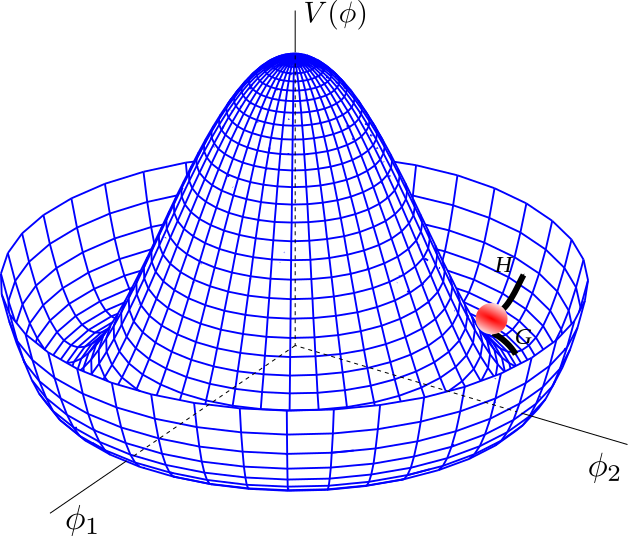
\includegraphics[scale=0.5]{mexicanhat}
  \caption{Potential for complex scalar field}
  \label{fig:mexicanhat}
\end{figure}



El Lagrangiano escalar complejo es equivalente al Lagragiano de dos campos escalares reales con los mismos paramétros. Para un conjunto de $N$ campos reales tenedremos (suma sobre $i$) \cite{Peskin}\footnote{\S 11.1}: 
\begin{align}
  \mathcal{L}=\frac{1}{2}\partial^\mu\phi^i\partial_\mu\phi_i-\frac{1}{2}\mu^2\phi_i\phi^i-\frac{1}{2}\mu^2\left(\phi_i\phi^i\right)^2\,,
\end{align}
que es invariante bajo una simetría $O(N)$
\begin{align}
  \phi^i\to{\phi'}^i=R^{ij}\phi^j\,,
\end{align}
para cualquier matriz $N\times  N$ ortogonal $R$. El análisis para $N=2$ da lugar a un bosón de Goldstone. El anális para $N>2$ es el mismo y por cada campo real que se introduzca aparece un nuevo bosón de Goldstone \cite{Peskin}:
\begin{quote}
  [\ldots] there are not continuous symmetries for $N=1$, while for $N=2$ there is a single direction of rotation. A rotation in $N$ dimensions can be in any one of $N(N-1)$ planes, so the $O(N)$--symmetric theory has $N(N-1)/2$ continuous symmetries. After spontaneous symmetry breaking there are $(N-1)(N-2)/2$  remaining symmetries corresponding to rotations of the $(N-1)$ [non massive] fields. The number of \emph{broken} symmetries is the difference, $N-1$.
\end{quote}
Entonces tenemos el siguiente teorema \cite{Peskin}
\begin{quote}
\emph{Goldstone's theorem states that for every spontaneously broken continuous symmetry, the theory must contain a massless particle.}
\end{quote}

Also from \cite{Peskin}\footnote{Introduction to Chapter 20}
\begin{quote}
  In a global symmetry  that is spontaneously broken the symmetry currents are still conserved and interactions are similarly restricted [the Lagrangian keeps the symmetry], but the vacuum state does not respect the symmetry and the particles do not form obvious symmetry multiplets. Instead, such a theory contains massless particles, Goldstone bosons, one for each generator of the spontaneously broken symmetry. The third case is that of a local, or gauge, symmetry. [\ldots] such a symmetry requires the existence of a massless vector field for each symmetry generator, and the interactions among these fields are highly restricted.

It is now only natural to consider a fourth possibility: What happens if we include both local gauge invariance  and spontaneous symmetry breaking in the same theory?
\end{quote}
 
\section{Principio gauge local}



En el caso de la Acción invariante gauge local bajo el Grupo $U(1)$, tenemos el Lagrangiano 
\begin{equation}
  \label{eq:89qft}
  \mathcal{L}=\left(\mathcal{D}^\mu\phi\right)^*\mathcal{D}_\mu\phi-\mu^2\phi^*\phi-\lambda\left(\phi^*\phi\right)^2-\tfrac{1}{4}F^{\mu\nu}F_{\mu\nu}
  \qquad 
  \mu^2\lt 0\text{ and } \lambda\gt 0\,.
\end{equation}
donde
\begin{align}
  \mathcal{D}_{\mu}=\partial_{\mu}+iq A_{\mu}\,.
\end{align}

Este es el Lagrangiano más general posible para un campo escalar complejo y el campo $A_\mu$ que deja la Acción invariante de Lorentz e invariante bajo la transformación gauge $U(1)$
\begin{align}
\label{eq:sqedgu}
  \phi(x)\to \phi'(x)=e^{i\theta(x)} \phi(x)\,,
\end{align}
En el caso de la superconductividad  electromagnético, $\phi$ representaría al campo escalar asociado al par de Cooper con carga eléctrica $-2$. Claramente el Lagrangiana en la ec.~\eqref{eq:89qft} es invariante local bajo tal $U(1)$ de carga eléctrica. 


\subsection{Gauge unitario}
Como $\phi$ es un campo complejo, podemos escribirlo en coordenadas polares con un campo real asociado a la magnitud del campo complejo y otro a la fase
\begin{align*}
  \phi(x)=\varphi(x)e^{i\eta(x)}
\end{align*}
Expandiendo el campo $\varphi(x)$ alrededor del mínimo: $\varphi(x)=(H(x)+v)/\sqrt{2}$, tenemos
\begin{align*}
    \phi(x)=e^{i\eta(x)}\left(\frac{H(x)+v}{\sqrt{2}}\right)\,.
\end{align*}


La libertad gauge nos permite en un momento determinado escoger la fase $\theta(x)$ de la ec.~\eqref{eq:sqedgu} sin que ese alteren los observables de la teoría. Para el campo en coordenadas polares tenemos que
\begin{align*}
     \phi\to\phi'=e^{i\theta(x)}e^{i\eta(x)}\left(\frac{H(x)+v}{\sqrt{2}}\right)
\end{align*}
Haciendo $\theta(x)=-\eta(x)$,
\begin{align}
\label{eq:87qft}
   \phi\to\phi'=&e^{-i\eta(x)+i\eta(x)}\left(\frac{H(x)+v}{\sqrt{2}}\right)=\frac{H(x)+v}{\sqrt{2}} \nonumber\\
   A_{\mu}\to A_{\mu}'=&A_{\mu}-\frac{1}{q}\partial_{\mu}\theta(x)\,.
\end{align}
\begin{align}
  \mathcal{L}\to\mathcal{L}' &=\left[\left(\mathcal{D}^\mu\right)'\phi'\right]^*\left(\mathcal{D}_\mu\right)'\phi'-\mu^2\left(\phi^*\right)'\phi'-\lambda\left[\left(\phi^*\right)'\phi'\right]^2-\tfrac{1}{4}\left(F^{\mu\nu}F_{\mu\nu}\right)'\nonumber\\
 &=\tfrac{1}{2}\left[\partial^\mu H+ig{A'}^\mu(H+v)\right]\left[\partial_\mu H-ig{A'}_\mu(H+v)\right]-\tfrac{1}{2}\mu^2(H+v)^2-\tfrac{1}{4}\lambda(H+v)^4-\tfrac{1}{4}\left(F^{\mu\nu}F_{\mu\nu}\right)'\,.
\end{align}

En adelante omitiremos las primas, aunque debe estar claro que se esta trabajando en el gauge específico de la ec.~\eqref{eq:87qft}. Entonces
\begin{align}
  \mathcal{L}&=\tfrac{1}{2}\partial^\mu H\partial_\mu H-\tfrac{1}{2}\mu^2(H+v)^2-
  \tfrac{1}{4}\lambda(H+v)^4+\tfrac{1}{2}g^2A^\mu A_\mu(H+v)^2
  -\tfrac{1}{4}F^{\mu\nu}F_{\mu\nu}.
\end{align}
Usando la ec.~\eqref{eq:84qft}
\begin{equation}
  \label{eq:94qft}
  \mathcal{L}=\mathcal{L}_H+\mathcal{L}_{A^\mu}+\tfrac{1}{2}g^2A^\mu A_\mu H^2+g^2vA^\mu A_\mu H,
\end{equation}
donde $\mathcal{L}_H$ esta dado por la ec.~\eqref{eq:88qft} y
\begin{equation}
  \mathcal{L}_{A^\mu}=-\tfrac{1}{4}F^{\mu\nu}F_{\mu\nu}+\tfrac{1}{2}g^2v^2A^\mu A_\mu.
\end{equation}
Teniendo en cuenta la ec.~\eqref{eq:23qft} para el Lagrangiano de Proca, vemos que como consecuencia de la ruptura espontánea de simetría el campo gauge ha adquirido una masa
\begin{equation}
  m_{A^\mu}=gv.
\end{equation}

El mecanismo completo mediante el cual, a partir de un Lagrangiano invariante gauge local, los bosones gauge adquieren masa se llama \emph{mecanismo de Brout–Englert–Higgs} \cite{Englert:1964et,Higgs:1964pj}. La partícula escalar que adquiere masa se llama Higgs, mientras que el bosón de Goldstone es absorbido por campo gauge como modo longitudinal. 

El número de grados de libertad independientes en el Lagrangiano original en la ec.~\eqref{eq:89qft} es cuatro. Correspondientes a los dos grados de libertad del bosón gauge no masivo y los dos del campo escalar complejo. En el Lagrangiano final en la ec.~\eqref{eq:94qft} no aparece el bosón de Goldstone. Sin embargo esto no es un problema porque dicho Lagrangiano también tiene cuatro grados de libertad correspondientes a  los tres grados de libertad del bosón gauge masivo y al grado de libertad del bosón de Higgs. 



\subsection{Superconductivity}

El campo $H$ dentro del superconductor, que hereda la carga $-2$ de
$\phi$, rompe espontáneamente carga eléctrica para esa configuración
especial del vacío (mínimo de energía) donde se forma el condensado de
pares de Cooper. Pero el la acción claramente conserva en todo momento
la carga eléctrica.

A review ot the use of the Proca Equations for a massive photon in superconductivity is given in~\cite{massivephoton}. A popularization review along this lines is in the book of Frank Wilczek ``The Lightness of Being'' (see Additional references).

The photon mass inside a superconductor is $10^{-11}\,$GeV (or 1/1000 of the electron mass according to~\cite{massivephoton}). Also from the article in Beamline $\lambda\sim 10\ \mu\text{m}$ y $M_\gamma=\hbar/\lambda c$ %check numbers

There are two important length scales in a superconductor. The first measures how efficientrly the condensate expels a magnetic field. In fact, the expulsion is not 

Additional references:
\begin{itemize}
\item The Lightness of Being: Mass, Ether, and the Unification of Forces,
Frank Wilczek, \url{http://www.amazon.com/The-Lightness-Being-Unification-Forces/dp/0465018955}
\item \url{http://www.scholarpedia.org/article/Englert-Brout-Higgs-Guralnik-Hagen-Kibble_mechanism_(history)}
\item Elementary Particle Physics: Volume 1: Quantum Field Theory and ..., Volume 1
 By Yorikiyo Nagashima, \url{Elementary Particle Physics: Volume 1: Quantum Field Theory and ..., Volume 1
 By Yorikiyo Nagashima}
\item From Superconductors 
to Supercolliders
by LANCE DIXON \url{http://www.slac.stanford.edu/pubs/beamline/26/1/26-1-dixon.pdf}
\item Electrodynamics of Superconductors \url{http://www.physics.buffalo.edu/phy514/w11/index.html}
\item Observan el análogo a un bosón de Higgs en un superconductor \url{http://francis.naukas.com/2014/09/05/analogo-al-boson-de-higgs-en-un-superconductor/}
\end{itemize}


%\left(\right)
%%% Local Variables: 
%%% mode: latex
%%% TeX-master: "fullnotes"
%%% ispell-local-dictionary: "castellano8"
%%% End: 
